% Gallery figure source
% Summary: An ancestral recombination graph. Backward in time, coalescence merges ancestral lineages and recombination splits one lineage into two parental lineages. The small bars indicate which genome intervals are carried by each lineage: blue intervals remain ancestral to sampled sequences, gray intervals are not ancestral to the samples, and orange intervals have already found a common ancestor for their local tree.
\documentclass[tikz,border=6pt]{standalone}
% Shared color palette
\usepackage[T1]{fontenc}
\usepackage[utf8]{inputenc}
\usepackage{lmodern}
\usepackage{microtype}
\usepackage{amsmath,amssymb,mathtools}
\usepackage{xcolor}
\usepackage{tikz}
\usetikzlibrary{arrows.meta,positioning,calc,fit,backgrounds,decorations.pathreplacing,shapes.geometric,shadows.blur}

\definecolor{mainblue}{RGB}{42,85,132}
\definecolor{deepgreen}{RGB}{30,105,70}
\definecolor{burntorange}{RGB}{190,90,25}
\definecolor{softgray}{RGB}{245,246,248}
\definecolor{darkgray}{RGB}{70,70,70}
\definecolor{violet}{RGB}{110,70,150}

\newcommand{\given}{\,|\,}
\newcommand{\Ne}{N_{e}}
\newcommand{\ARG}{\mathrm{ARG}}
\newcommand{\MRCA}{\mathrm{MRCA}}
\newcommand{\GMRCA}{\mathrm{GMRCA}}

% Shared TikZ styles
\tikzset{
  tip/.style={circle,fill=black,inner sep=1.6pt},
  nodept/.style={circle,fill=black,inner sep=1.4pt},
  sampled/.style={rectangle,fill=black,inner sep=2.2pt},
  branch/.style={line width=0.8pt},
  retic/.style={circle,draw=burntorange,fill=burntorange!25,line width=0.8pt,inner sep=2.0pt},
  event/.style={circle,draw=mainblue,fill=mainblue!15,line width=0.8pt,inner sep=1.8pt},
  arr/.style={-{Latex[length=2.0mm]},line width=0.8pt},
  faint/.style={line width=0.7pt,draw=gray!55},
  parentedge/.style={-{Latex[length=2.0mm]},line width=0.9pt,draw=burntorange},
  treeedge/.style={-{Latex[length=2.0mm]},line width=0.9pt,draw=black},
  segment/.style={line width=4pt,line cap=round},
  dashedretic/.style={-{Latex[length=2.0mm]},line width=0.9pt,draw=burntorange,dashed}
}


\begin{document}
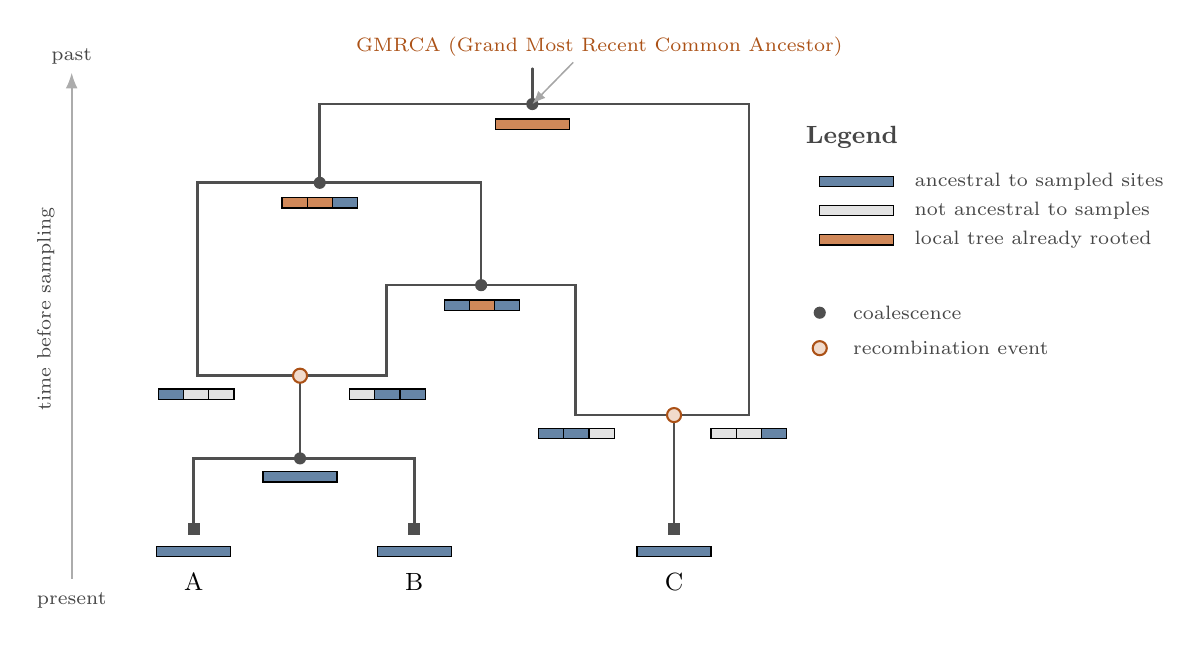
\begin{tikzpicture}[
  scale=1.0,
  argedge/.style={line width=.95pt,draw=darkgray!95,line cap=round},
  seqframe/.style={draw=black,line width=.45pt},
  seqbarlabel/.style={font=\scriptsize,align=left,text=darkgray},
  timelabel/.style={font=\scriptsize,text=darkgray},
  coalevent/.style={circle,fill=darkgray!95,inner sep=1.55pt},
  recombevent/.style={circle,draw=burntorange!90!black,fill=burntorange!22,line width=.75pt,inner sep=1.8pt},
  samplebox/.style={rectangle,fill=darkgray!95,inner sep=2.1pt},
  callout/.style={font=\scriptsize,align=center,text=darkgray},
  callarr/.style={-{Latex[length=1.7mm]},line width=.55pt,draw=gray!70}
]

  \def\seqFull#1#2#3{%
    \begin{scope}[shift={(#1,#2)}]
      \draw[seqframe,fill=#3] (0,0) rectangle (.94,.13);
    \end{scope}%
  }

  \def\seqThree#1#2#3#4#5{%
    \begin{scope}[shift={(#1,#2)}]
      \draw[seqframe,fill=#3] (0,0) rectangle (.32,.13);
      \draw[seqframe,fill=#4] (.32,0) rectangle (.64,.13);
      \draw[seqframe,fill=#5] (.64,0) rectangle (.96,.13);
    \end{scope}%
  }

  \draw[-{Latex[length=2mm]},draw=gray!65,line width=.7pt]
    (-0.35,-0.28)--(-0.35,6.15);

  \node[timelabel,rotate=90] at (-0.68,3.15)
    {time before sampling};
  \node[timelabel] at (-0.35,6.35) {past};
  \node[timelabel] at (-0.35,-0.55) {present};

  \coordinate (SA) at (1.20,0.35);
  \coordinate (SB) at (4.00,0.35);
  \coordinate (SC) at (7.30,0.35);

  \coordinate (cAB)  at (2.55,1.25);
  \coordinate (rOne) at (2.55,2.30);
  \coordinate (rTwo) at (7.30,1.80);

  \coordinate (cMid)  at (4.85,3.45);
  \coordinate (cMidL) at (3.65,3.45);
  \coordinate (cMidR) at (6.05,3.45);

  \coordinate (cTop)  at (2.80,4.75);
  \coordinate (cTopL) at (1.25,4.75);
  \coordinate (cTopR) at (4.00,4.75);

  \coordinate (g)  at (5.50,5.75);
  \coordinate (gL) at (2.80,5.75);
  \coordinate (gR) at (8.25,5.75);

  \draw[argedge] (SA)--(1.20,1.25)--(cAB);
  \draw[argedge] (SB)--(4.00,1.25)--(cAB);
  \draw[argedge] (cAB)--(rOne);

  \draw[argedge] (rOne)--(1.25,2.30)--(1.25,4.75)--(cTopL)--(cTop);
  \draw[argedge] (rOne)--(3.65,2.30)--(3.65,3.45)--(cMidL)--(cMid);

  \draw[argedge] (SC)--(rTwo);
  \draw[argedge] (rTwo)--(6.05,1.80)--(6.05,3.45)--(cMidR)--(cMid);
  \draw[argedge] (rTwo)--(8.25,1.80)--(8.25,5.75)--(gR)--(g);

  \draw[argedge] (cMid)--(4.85,4.75)--(cTopR)--(cTop);
  \draw[argedge] (cTop)--(gL)--(g);
  \draw[argedge] (g)--(5.50,6.20);

  \node[coalevent] at (cAB) {};
  \node[recombevent] at (rOne) {};
  \node[recombevent] at (rTwo) {};
  \node[coalevent] at (cMid) {};
  \node[coalevent] at (cTop) {};
  \node[coalevent] at (g) {};

  \node[samplebox] at (SA) {};
  \node[samplebox] at (SB) {};
  \node[samplebox] at (SC) {};

  \node[font=\small] at (1.20,-0.32) {A};
  \node[font=\small] at (4.00,-0.32) {B};
  \node[font=\small] at (7.30,-0.32) {C};


  \seqFull{0.73}{-0}{mainblue!72}
  \seqFull{3.53}{-0}{mainblue!72}
  \seqFull{6.83}{-0}{mainblue!72}

  \seqFull{2.08}{0.95}{mainblue!72}

  \seqThree{0.75}{2.0}{mainblue!72}{gray!22}{gray!22}
  \seqThree{3.18}{2.0}{gray!22}{mainblue!72}{mainblue!72}

  \seqThree{5.58}{1.50}{mainblue!72}{mainblue!72}{gray!22}
  \seqThree{7.77}{1.50}{gray!22}{gray!22}{mainblue!72}

  \seqThree{4.38}{3.13}{mainblue!72}{burntorange!72}{mainblue!72}

  \seqThree{2.32}{4.43}{burntorange!72}{burntorange!72}{mainblue!72}

  \seqFull{5.03}{5.43}{burntorange!72}

  \begin{scope}[xshift=9.15cm,yshift=4.55cm]
    \node[font=\small\bfseries,text=darkgray,anchor=west] at (-0.3,0.78)
      {Legend};

    \seqFull{0}{0.15}{mainblue!72}
    \node[seqbarlabel,anchor=west] at (1.08,0.22)
      {ancestral to sampled sites};

    \seqFull{0}{-0.22}{gray!22}
    \node[seqbarlabel,anchor=west] at (1.08,-0.15)
      {not ancestral to samples};

    \seqFull{0}{-0.59}{burntorange!72}
    \node[seqbarlabel,anchor=west] at (1.08,-0.52)
      {local tree already rooted};
  \end{scope}

  \begin{scope}[xshift=9.15cm,yshift=2.85cm]
    \node[coalevent] at (0,0.25) {};
    \node[seqbarlabel,anchor=west] at (.30,0.25)
      {coalescence};

    \node[recombevent] at (0,-0.20) {};
    \node[seqbarlabel,anchor=west] at (.30,-0.20)
      {recombination event};
  \end{scope}

  \node[callout,text=burntorange!90!black] (GMRCA) at (6.35,6.48) {GMRCA (Grand Most Recent Common Ancestor)};
  \draw[callarr] (6.02,6.28)--(g);

\end{tikzpicture}
\end{document}
